\section{Method}
\chead{\thesection. Method}

The primary objective of this work is to compare two MCL-based clustering
methods on large-scale protein sequence datasets using Protein Sequence
Similarity Networks (PSSNs). The adopted workflow follows the CGG Toolkit
\cite{cggToolkit} framework and its flow diagram is illustrated in
Fig.~\ref{fig:workhigh}. Along with the clustering analysis, a qualitative study
is performed to characterize each dataset, including frequency diagrams of
residue distributions and sequence lengths, as well as heatmaps of adjacency
matrices.

Initially, protein sequences are curated using a standardized preprocessing
pipeline to ensure unique sequence identification. Low-complexity sequence
regions are then masked to prevent bias in subsequent sequence similarity
scoring. Masking low-complexity regions is a standard preprocessing step to
avoid spurious sequence similarity matches \cite{wootton1996seg}. After
applying a local sequence aligner, the computed sequence scores are used to
construct a PSSN. In the resulting graph, vertices correspond to protein
sequences and weighted edges encode pairwise similarity.

The primary contribution lies in the application and comparison of
reproducible, interpretable and scalable flow-based graph clustering methods,
specifically the Markov Cluster Algorithm (MCL) and its high performance
variant HipMCL, to cluster the produced PSSN into groups of homologous
proteins. The comparison evaluates each method's computational feasibility in
terms of peak memory usage and runtime in a single node, providing insight into
their scalability on large-scale protein sequence datasets.

% 600%
\begin{figure}[htbp]
  \centering
  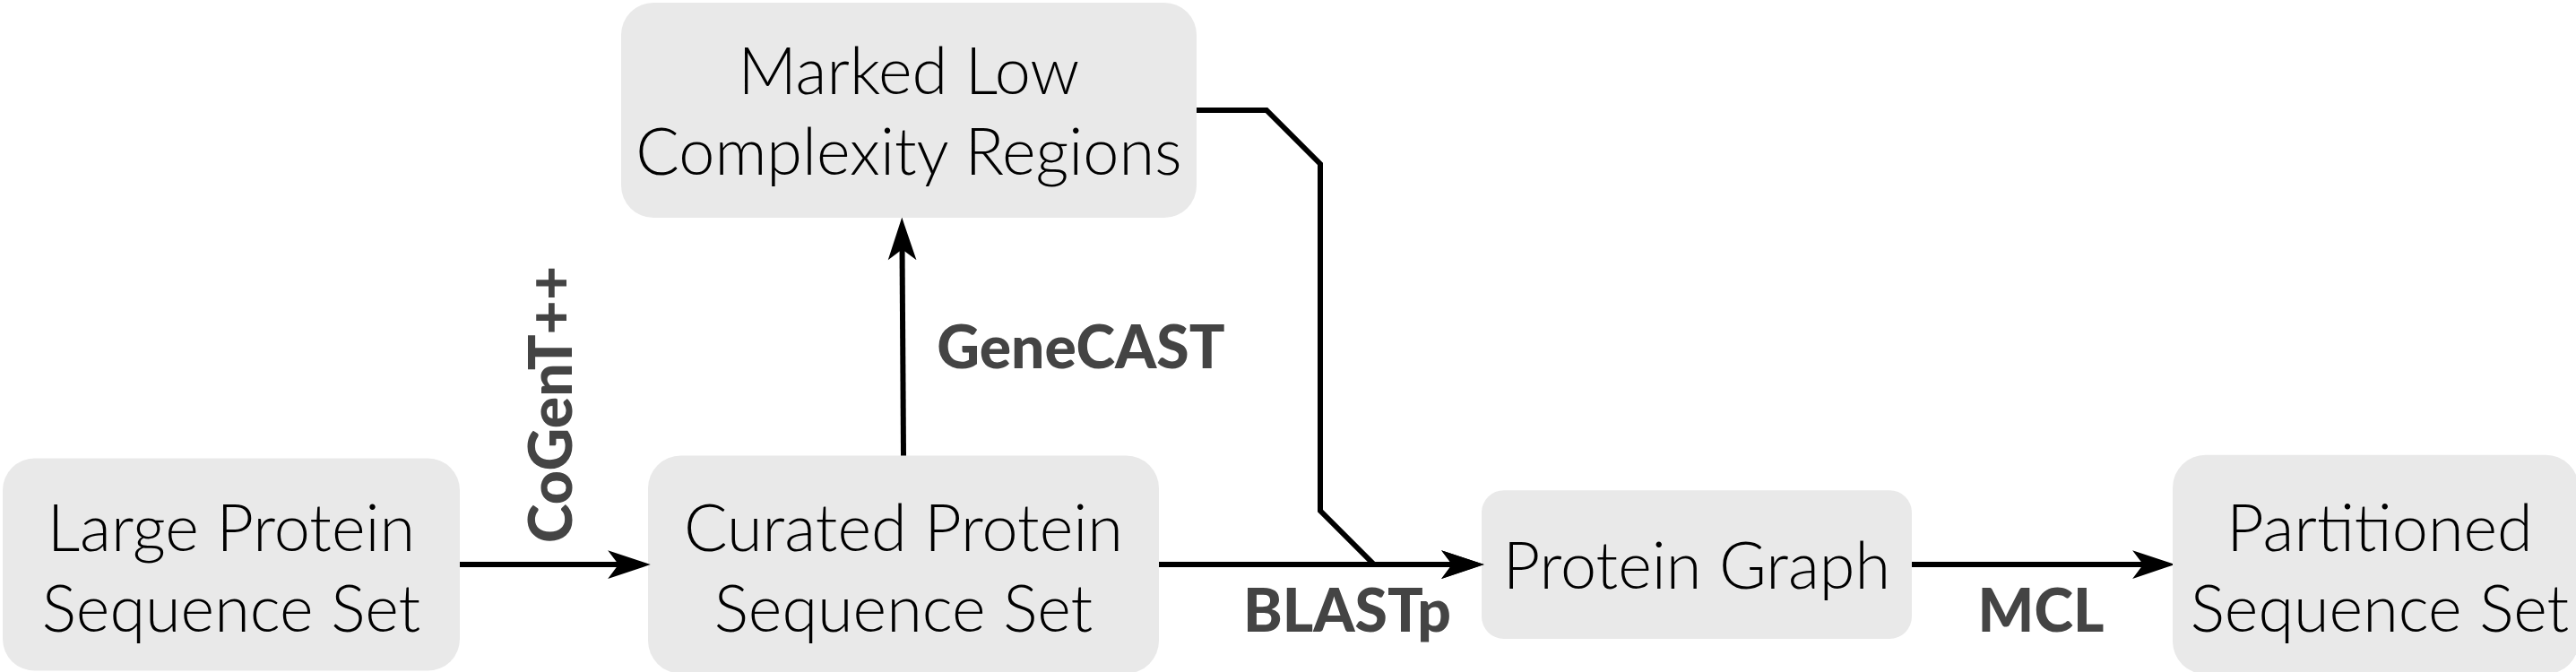
\includegraphics[width=1\linewidth]{asset/workhigh.png}
  \caption{Overview of the protein clustering workflow based on the CGG Toolkit. Each node represents a data object, and each directed edge denotes a transformation.}
  \label{fig:workhigh}
\end{figure}

\subsection{Data}

\subsubsection{Raw Data}

The data used in this project were protein sequences obtained from UniProt
\cite{uniprot}, a comprehensive repository maintained by the European
Bioinformatics Institute (EBI), the SIB Swiss Institute of Bioinformatics, and
the Protein Information Resource (PIR). For this thesis, the datasets were
drawn from UniProtKB, one of the three major database resources of UniProt.
Specifically, a large collection of FASTA records was obtained from UniProtKB
release 2025 April 02. Since the current work is limited to the analysis of
protein molecules, non-protein data (e.g., nucleic
acid sequences) were discarded. The final parsed dataset consists entirely of
curated \textit{reference proteomes}.

Reference proteomes are representative, non-redundant sets of protein sequences
selected to cover well-studied model organisms and species of biomedical or
phylogenetic interest. Each reference proteome includes canonical protein
sequences and, where available, additional isoforms or variant sequences, all
provided in standard FASTA format. Therefore, the raw data consists
exclusively of protein FASTA files obtained from the UniProt FTP
repository\footnote{\url{https://ftp.uniprot.org/pub/databases/uniprot/previous_major_releases/release-2025_02}}.
Viral reference proteomes were excluded to maintain taxonomic consistency, as
viruses differ fundamentally from cellular organisms in their evolutionary
patterns, and protein sequence characteristics. After discarding the viral proteomes, the distribution of obtained sequences per superkingdom is displayed in Table~\ref{tab:superkingdomDistribution}.

\begin{table}[htbp]
	\centering
	\caption{Distribution of proteomes and protein records in UniProtKB by taxonomic superkingdom.}
	\begin{tabular}{ccc}
		\toprule
		\textbf{Superkingdom} & \textbf{\# Proteomes} & \textbf{\# Protein Records} \\
		\midrule
		\arrayrulecolor{gray!50}
		Archaea & 303 & 750,976 \\
    \midrule
		Bacteria & 9,084 & 35,298,460 \\
		\midrule
		Eukaryota & 2,740 & 46,079,603 \\
		\arrayrulecolor{black}
		\midrule
		\textbf{Total} & 12,127 & 82,129,039 \\
    \bottomrule
	\end{tabular}
	\label{tab:superkingdomDistribution}
\end{table}

\subsubsection{FASTA Format}

Protein sequences were provided in standard FASTA format, a plain-text
representation for biological sequences. Each FASTA record consists of a single
header line followed by one or more lines encoding the sequence. 

Specifically, a FASTA record has the following format:

\begin{plaintext}
>HEADER[|DESCRIPTION]
SEQ_BLOCK
\end{plaintext}

\begin{table}[htbp]
	\centering
	\caption{Components of any FASTA record.}
	\begin{tabular}{p{3cm} p{10cm}}
		\toprule
		\textbf{Placeholder} & \textbf{Description} \\
    \midrule
		\texttt{HEADER} & A sequence identifier. Its syntax and semantics are database-specific (e.g., UniProt), and uniqueness is guaranteed only within the originating database. \\
		\arrayrulecolor{gray!50}
    \midrule
		\texttt{|DESCRIPTION} & Optional field. \texttt{|} is a literal character. Additional annotation fields, typically separated by spaces or pipe (\texttt{|}) characters, providing metadata such as protein name or organism. \\
		\midrule
		\texttt{SEQ\_BLOCK} & The biological sequence encoded using single-letter residue codes. Sequence lines may be wrapped and are interpreted as a contiguous sequence. \\
		\arrayrulecolor{black}
    \bottomrule
	\end{tabular}
	\label{tab:fastaComponents}
\end{table}

Observe Table~\ref{tab:fastaComponents} for the semantics of each component of
the aforementioned formatting. A FASTA file may contain more than one record.
FASTA files in this study contain protein sequences only. Common file
extensions include \texttt{.fasta}, \texttt{.fa}, and \texttt{.faa}.

\subsubsection{Curated Data}

The protein sequences obtained from UniProtKB were further processed based on
the CoGenT++ \cite{cogent0, cogent1} format to produce a curated dataset for
downstream tasks such as clustering. This process of curation involves the
systematic prefixing and standardization of the FASTA header. It ensures
uniqueness across all sequences using a compact identifier while encoding
additional globally identifiable metadata in a consistent format, while
preserving the initial header of the raw FASTA record.

Each FASTA record that is subjected to this curation follows the template:

\begin{plaintext}
>PROTEOMEID-TAXID-TRUNC_NAME-YEAR-PROT_CNT-SUPERKINGDOM-SEQ_CNT OLD_ID[|DESCRIPTION]
SEQ_BLOCK
\end{plaintext}

The following example is a FASTA record after being subjected to CoGenT++
curation, holding the protein called \textit{Chemokine-like Factor}. It
represents a sequence of amino acid residues originating from the human
proteome.

\begin{table}
  \centering
  \caption{Components of a CoGenT++ curated FASTA record.}
  \begin{tabular}{p{3cm} p{7cm} p{4.3cm}}
		\toprule
		\textbf{Placeholder} & \textbf{Description} & \textbf{Example} \\
    \midrule
		\texttt{PROTEOMEID} & UniProt reference proteome identifier. Each corresponds to exactly one \texttt{TAXID}. & \texttt{UP000005640} \\
		\arrayrulecolor{gray!50}
		\midrule
		\texttt{TAXID} & 8-digit zero-padded NCBI taxonomy ID of the source organism. & \texttt{00009606} \\
		\midrule
		\texttt{TRUNC\_NAME} & Truncated protein or gene name derived from the original header. & \texttt{Homo\_sapi} \\
		\midrule
		\texttt{YEAR} & Dataset release year or batch number. & \texttt{26} \\
		\midrule
		\texttt{PROT\_CNT} & 6-digit zero-padded per-superkingdom sequence counter starting from \texttt{000001}. & \texttt{000594} \\
		\midrule
		\texttt{SUPERKINGDOM} & Single-letter code for proteome's superkingdom (A = Archaea, B = Bacteria, E = Eukaryota). & \texttt{E} \\
		\midrule
		\texttt{SEQ\_CNT} & 6-digit zero-padded per-proteome sequence counter starting from \texttt{000001}. & \texttt{000996} \\
		\midrule
		\texttt{OLD\_ID} & Original UniProt FASTA identifier, preserved for traceability. & \texttt{sp|Q9UBR5|CKLF\_HUMAN} \\
		\midrule
		\texttt{|DESCRIPTION} & Optional metadata from the original header. & \texttt{Chemokine\dots SV=1} \\
		\midrule
		\texttt{SEQ\_BLOCK} & Amino-acid sequence, identical to the raw data. & See FASTA sequence. \\
		\arrayrulecolor{black}
    \bottomrule
  \end{tabular}
  \label{tab:curatedFastaComponents}
\end{table}

\begin{plaintext}
>UP000005640-00009606-Homo_sapi-26-000594-E-000996 sp|Q9UBR5|CKLF_HUMAN Chemokine-like factor OS=Homo sapiens OX=9606 GN=CKLF PE=1 SV=1
MDNVQPKIKHRPFCFSVKGHVKMLRLALTVTSMTFFIIAQAPEPYIVITGFEVTVILFFI
LLYVLRLDRLMKWLFWPLLDIINSLVTTVFMLIVSVLALIPETTTLTVGGGVFALVTAVC
CLADGALIYRKLLFNPSGPYQKKPVHEKKEVL
\end{plaintext}

Observe Table~\ref{tab:curatedFastaComponents} for the semantics of each
component of the aforementioned formatting. All sequences and headers remain
consistent with the FASTA format without disposing UniProt's annotations. These
principles are designed to facilitate reproducible, transferable and scalable
biological sequence analysis workflows such as the one outlined in the project
of the CGG Toolkit, making it suitable for the current protein analysis
workflow (observe Fig.~\ref{fig:workhigh}).

The resulting dataset will be referred to as \texttt{ref\_prot} throughout this study. Additionally, subsets of \texttt{ref\_prot} are isolated to investigate
\begin{itemize}
  \item The computational requirements of the clustering workflow, or
  \item A qualitative analysis of specific organisms.
\end{itemize}
In total, 13 additional subsets of \texttt{ref\_prot} were separately
analysed (observe Table~\ref{tab:dataStats}). It is worth noting that not all
pairs of these subsets are disjoint. Also, each dataset is assigned an
identifier. For each of these datasets, the identifier will be used as a
basename for all files tied to it, e.g., for the dataset
\texttt{ref\_prot}, its FASTA file is named as
\texttt{ref\_prot.fasta} and its partition \texttt{ref\_prot.cl}.

\begin{table}[htbp]
  \centering
  \caption{Subsets of \texttt{ref\_prot}. The column \textbf{Cmp} refers to whether that subset was utilized for the clustering analysis, while \textbf{Qlt} refers to qualitative analysis. Also, \textbf{Seq Len} and \textbf{Rec Cnt} refer to the protein length and record count corresponding to the length that appears most frequently. Finally, the \textbf{Size} column lists the number of records per dataset.}
  \begin{tabular}{ccc cc cc}
    \toprule
    \multicolumn{3}{c}{\textbf{General Data Information}} & \multicolumn{2}{c}{\textbf{Most Freq Length}} & \multicolumn{2}{c}{\textbf{Analysis}} \\
    \arrayrulecolor{gray!50}
    \midrule
    \arrayrulecolor{black}
    \textbf{Identifier} & \textbf{Size} & \textbf{Tax ID} & \textbf{Seq Len} & \textbf{Rec Cnt} & \textbf{Cmp} & \textbf{Qlt} \\
    \midrule
    \texttt{homo\_sapi} & 20,647 & 00009606 & 117 & 109 & \ding{51} & \ding{51} \\
    \arrayrulecolor{gray!50}
    \midrule
    \texttt{arab\_thal} & 27,448 & 00003702 & 256 & 75 & \textcolor{gray}{\ding{53}} & \ding{51} \\
    \midrule
    \texttt{carn\_malt} & 3,539 & 01234679 & 216 & 19 & \textcolor{gray}{\ding{53}} & \ding{51} \\
    \midrule
    \texttt{dani\_reri} & 26,728 & 00007955 & 257 & 70 & \textcolor{gray}{\ding{53}} & \ding{51} \\
    \midrule
    \texttt{sacc\_cere} & 6,065 & 00559292 & 440 & 40 & \textcolor{gray}{\ding{53}} & \ding{51} \\
    \midrule
    \texttt{hds\_prot} & 53,440 & \textcolor{gray}{N/A} & 312 & 155 & \ding{51} & \ding{51} \\
    \midrule
    \texttt{hac\_prot} & 51,634 & \textcolor{gray}{N/A} & 117 & 168 & \ding{51} & \ding{51} \\
    \midrule
    \texttt{hac\_prot\_small} & 18,002 & \textcolor{gray}{N/A} & \textcolor{gray}{N/A} & \textcolor{gray}{N/A} & \textcolor{gray}{\ding{53}} & \ding{51} \\
    \midrule
    \texttt{hds\_prot\_small} & 22,547 & \textcolor{gray}{N/A} & \textcolor{gray}{N/A} & \textcolor{gray}{N/A} & \textcolor{gray}{\ding{53}} & \ding{51} \\
    \midrule
    \texttt{archaea\_medium} & 378,303 & \textcolor{gray}{N/A} & \textcolor{gray}{N/A} & \textcolor{gray}{N/A} & \ding{51} & \textcolor{gray}{\ding{53}} \\
    \midrule
    \texttt{archaea} & 750,976 & \textcolor{gray}{N/A} & \textcolor{gray}{N/A} & \textcolor{gray}{N/A} & \ding{51} & \textcolor{gray}{\ding{53}} \\
    \midrule
    \texttt{bacteria\_tiny} & 2,972 K & \textcolor{gray}{N/A} & \textcolor{gray}{N/A} & \textcolor{gray}{N/A} & \ding{51} & \ding{51} \\
    \midrule
    \texttt{bacteria} & 35,298 K & \textcolor{gray}{N/A} & \textcolor{gray}{N/A} & \textcolor{gray}{N/A} & \ding{51} & \textcolor{gray}{\ding{53}} \\
    \midrule
    \texttt{ref\_prot} & 82,129 K & \textcolor{gray}{N/A} & \textcolor{gray}{N/A} & \textcolor{gray}{N/A} & \ding{51} & \textcolor{gray}{\ding{53}} \\
    \arrayrulecolor{black}
    \bottomrule
  \end{tabular}
  \label{tab:dataStats}
\end{table}

The first five datasets of Table~\ref{tab:dataStats} are individual reference
proteomes: \texttt{homo\_sapi}, \texttt{arab\_thal}, \texttt{carn\_malt},
\texttt{dani\_reri}, and \texttt{sacc\_cere}. These correspond to human, plant,
bacterium, zebrafish, and yeast (fungus), respectively. These are collectively
used as a foundation for the qualitative analysis, since \texttt{hac\_prot},
\texttt{hds\_prot} are a concatenation of \(\{\)\texttt{homo\_sapi},
\texttt{arab\_thal}, \texttt{carn\_malt}\(\}\) and \(\{\)\texttt{homo\_sapi},
\texttt{dani\_reri}, \texttt{sacc\_cere}\(\}\), respectively. In the same
order, the sequence sets \texttt{hac\_prot\_small} and
\texttt{hds\_prot\_small} are subsets of the former pair, in a way that makes
the organism distribution more uniform for the similarity heatmaps.

\subsection{Graph-based Representation of Protein Sequences}

Protein sequences are variable-length symbolic objects defined over an amino
acid alphabet comprised of 20 monomeric units (observe Table~\ref{tab:amino_acids}). Since the current task is
to partition the sequence set \(\mathscr{V}\), we first construct a numerical
representation of the dataset. 

In this work, similarities are measured using BLASTp \cite{blast}, a widely used sequence aligner, through the
DIAMOND tool \cite{diamond}. We have utilized DIAMOND's git repository\footnote{\url{https://github.com/bbuchfink/diamond} from the codebase with commit hash \texttt{0x25165b5}.}. BLASTp performs local sequence alignment on protein sequences. In this case, BLASTp
utilizes the 20 x 20 substitution matrix called BLOSUM62 (observe the
\texttt{-{}-matrix} parameter) to perform the alignment. A substitution matrix is a symmetric matrix that defines
scores for aligning amino acid residue pairs based on observed evolutionary
substitution patterns, assigning positive scores to substitutions between
similar residues (e.g., Isoleucine and Leucine) and negative scores to unlikely
substitutions. BLASTp takes a pair of sequences as input and, after
sequence alignment, it produces a set of scores that express pairwise
similarity. Bulk processing is performed in an all-versus-all manner over
\(\mathscr{V}\), from which only the top 25 optimal alignment pairs are kept
(through \texttt{-{}-max-target-seqs}).
To model pairwise similarity, we use the maximum bit score that reflects the
strength of the match, independent of the input database. Another important output
value of BLASTp that is utilized is the input pair's E-value, a statistical
measure of the expected number of matches of similar quality that would occur
by chance when comparing against a database of reference proteins. A lower
E-value corresponds to a more statistically significant similarity, indicating
a stronger relationship of the corresponding sequence pair.

A known issue in local sequence alignment is the presence of low-entropy or
repeating patterns, which can lead to artificially inflated similarity scores.
For example, the subsequences \texttt{GGGGGG} and \texttt{PEPEPEPEPE} are
frequently encountered in existing protein sequences. Since sequence alignment is
performed locally, these may match many unrelated sequences solely due to
compositional bias, producing high maximum bit scores and low E-values despite
lacking evolutionary relatedness. Such motifs are called
\textit{low-complexity} and to mitigate the negative effect of their
repetition, sequences are preprocessed based on GeneCAST \cite{genecast}, an
algorithm that identifies and masks low-complexity regions prior to alignment.
The utilized implementation of GeneCAST relied on \texttt{genecast\_1}, a
specific tool originating from the official CGG Toolkit's
repository\footnote{\url{https://github.com/bcpl-certh/cgg-toolkit/tree/main/1_genecast}
at commit \texttt{0x92243d0}.}. The only parameter that is overridden is
\texttt{MAXSEQLEN} from the file \texttt{:/genecast\_1/cast.c}, which is set to
\texttt{50000}, since the input data contain sequences of length greater than
the default value. This parameter controls the maximum sequence length that can
be processed from the input sample. The rest of the configuration was preserved
to its default settings. Also, the masking is performed by simply replacing the
identified low-complexity local region with an equal length of multiple
\(\texttt{X}\) characters. The character \(\texttt{X}\) is a special token that
does not belong in the protein residue alphabet and is therefore unrecognizable
by BLASTp. For example, the motif \texttt{ASSSGAGAAAAAAAA} that appears in

\begin{plaintext}
>UP000005640-00009606-Homo_sapi-26-000594-E-000041 sp|Q08AG7... PE=1 SV=2
M$\texttt{\underline{ASSSGAGAAAAAAAA}}$NLNAVRETMDVLLEISRILNTGLDMETLSICVRLCEQGINPEAL
SSVIKELRKATEALKAAENMTS
\end{plaintext}

is subsequently localized by GeneCAST and classified as a low-complexity region relative to that specific sequence. Then, the sequence is modified into

\begin{plaintext}
>UP000005640-00009606-Homo_sapi-26-000594-E-000041 sp|Q08AG7... PE=1 SV=2 
M$\texttt{\underline{XSSSGXGXXXXXXXX}}$NLNAVRETMDVLLEISRILNTGLDMETLSICVRLCEQGINPEAL 
SSVIKELRKATEALKAAENMTS
\end{plaintext}

Subsequently, these low complexity regions do not contribute to the scoring of
a pair's alignment, as they always mismatch with the original residue tokens.
The masking is applied to the input FASTA file using the following command:
\begin{plaintext}[numbers=none]
cast sample.fasta > sample.casta
\end{plaintext}
after masking, an all‑vs‑all sequence alignment is performed with diamond:
\begin{plaintext}
diamond blastp --query sample.casta --db sample.fasta --out sample.pairs --outfmt 6 qseqid sseqid bitscore evalue
\end{plaintext}
from the raw alignments, only statistically significant pairs (e‑value \(\leq\) 0.005) are retained, extracting the query id, subject id, and bit score:
\begin{plaintext}[numbers=none]
awk '$\textdollar$(NF) <= 0.005 {print $\textdollar$1, $\textdollar$2, $\textdollar$(NF-1)}' sample.pairs > sample.adj
\end{plaintext}
After the dataset is processed by GeneCAST and BLASTp, the resulting pairwise
similarity matrix is further sparsified by filtering out statistically
insignificant weights. In this case, the filtering is performed by setting the
E-value cutoff to \(5 \cdot 10^{-3}\), effectively keeping only the edges that
correspond to E-values smaller than or equal to the selected cutoff value. This
produces a sparse similarity representation of protein pairs comprising only
statistically significant relationships. The resulting file \texttt{sample.adj}
is a compact representation of the adjacency matrix \(\mathcal{A}\) containing
only the identifiers of the preserved protein pairs along with their similarity
values. Thus, each line has the following simple structure \texttt{S1\_ID
S2\_ID BITSCORE\_1\_2}. To demonstrate with an example, what follows below is
a segment of three lines from the \texttt{homo\_sapi.adj} file
\begin{plaintext}
UP000005640-00009606-Homo_sapi-26-000594-E-000003 UP000005640-00009606-Homo_sapi-26-000594-E-002855 69.3
UP000005640-00009606-Homo_sapi-26-000594-E-000003 UP000005640-00009606-Homo_sapi-26-000594-E-001453 62.4
UP000005640-00009606-Homo_sapi-26-000594-E-000003 UP000005640-00009606-Homo_sapi-26-000594-E-003006 61.2
\end{plaintext}

\subsection{Clustering}

Up to this point, we have demonstrated how the sparse weighted adjacency matrix
\(\mathcal{A}\) was constructed and encoded in the file \texttt{sample.adj}.
Together with the sequence dataset \(\mathscr{V}\) encoded in
\texttt{sample.fasta}, this pair of files defines a sparse
PSSN, serving as the input to the protein clustering stage.

Clustering is performed using the Markov Cluster Algorithm (MCL). Two
implementations were evaluated: the reference MCL \cite{mcl} via the
\texttt{mcl}\footnote{\url{https://github.com/micans/mcl} at commit
\texttt{0x8c99282}.} CLI tool and its high-performance variant HipMCL \cite{hipmcl}
via the \texttt{hipmcl}\footnote{\url{https://bitbucket.org/azadcse/hipmcl} at
commit \texttt{0xca6a4fb}.} tool. Both methods operate directly on the
constructed PSSN and partition the vertex set into a collection of disjoint
graph clusters (communities). The resulting partition is exported to a file
named \texttt{sample.cl}.

\subsubsection{MCL}

For clustering with the reference MCL implementation, the graph is first converted to MCL's native matrix format using \texttt{mcxload}:

\begin{plaintext}[numbers=none]
mcxload --stream-mirror -abc sample.adj -o sample.mci -write-tab sample.tab
\end{plaintext}

Here, \texttt{-abc} specifies the aforementioned pair-edge format of
\texttt{sample.adj}. The flag \texttt{-{}-stream-mirror} enforces symmetric
loading of the edge list, and \texttt{-write-tab} stores the mapping between
sequence identifiers and internal matrix indices for later reference.

Clustering is then performed on the converted graph using \texttt{mcl}:

\begin{plaintext}[numbers=none]
mcl sample.mci -I INFLATION -te 48 -use-tab sample.tab -o sample.cl
\end{plaintext}

The \texttt{-te 48} flag requests 48 worker threads, half of the total number
of virtual threads available on the compute node (96). The \texttt{-I} parameter sets the inflation value, which indirectly controls the
granularity of the resulting partition. The output is written to
\texttt{sample.cl}, where each line contains a whitespace-separated list of
protein identifiers belonging to a single cluster.

\subsubsection{HipMCL}

Clustering was also performed with \texttt{HipMCL}. Since the present study is
restricted to a single compute node, \texttt{HipMCL} is not used in a
distributed multi-node configuration for which it was designed. Instead, it
is executed locally on the PSSN through the command

\begin{plaintext}[numbers=none]
hipmcl -M sample.adj -I INFLATION -per-process-mem 16 -o sample.cl
\end{plaintext}

where \texttt{-M} specifies the weighted graph input, \texttt{-I INFLATION} is
the inflation parameter, and \texttt{-per-process-mem 16} reserves 16~GiB of
memory per process. The output of \texttt{HipMCL} is a partition of the input
vertex set into disjoint clusters, analogous to the output of standard MCL.

\subsubsection{Output processing and recorded measurements}

The raw clustering output of each method consists of one line per cluster, with
sequence identifiers separated by whitespace. Clusters are listed in decreasing
order with respect to cluster size. For example, for a sequence set
\(\mathscr{V}\) with identifiers \(\{\)\texttt{S01\_ID}, \dots,
\texttt{S16\_ID}\(\}\), a valid \texttt{sample.cl} file might contain:

\begin{plaintext}
S01_ID S02_ID S03_ID S04_ID
S05_ID S06_ID S07_ID S08_ID
S09_ID S10_ID S11_ID
S12_ID S13_ID
S14_ID S15_ID
S16_ID
\end{plaintext}

This shows that the sequences corresponding to the identifier collection
\(\{\)\texttt{S01\_ID, ..., S04\_ID}\(\}\) is a single cluster, \(\{\)\texttt{S05\_ID, ..., S08\_ID}\(\}\) is another cluster, and so on.

\subsection[Workflow \& \ Streamlined Implementation]{Workflow \& Streamlined Implementation}

The low-complexity masking, alignment, filtering, PSSN construction, and its
partitioning steps described above were integrated into a single executable
workflow called
\texttt{bioscflow}\footnote{\url{https://github.com/fl0wxr/bioscflow} at commit \texttt{0xc81d4e6}.}. The
tool is implemented in Python and orchestrates the execution of external
dependencies (GeneCAST, DIAMOND, MCL, HipMCL) while managing file paths,
intermediate data, and result logging. The workflow is designed for single-node
execution.

\texttt{bioscflow} is invoked from the command line with the following required parameters:

\begin{plaintext}[numbers=none]
python3 run.py --db data/raw/sample.fasta -I INFLATION --algorithm mcl
\end{plaintext}

The full interface is summarized below:

\begin{plaintext}
usage: run.py [-h] --db DB -I I --algorithm {mcl,hipmcl} [--nopreproc] [--debug]

bioscflow: Perform community detection on a sequence similarity network. The vertex weight is set as the bit score estimated from an all-vs-all local sequence alignment (BLASTp), applied on some set of user provided database of FASTA sequences.

options:
  -h, --help            show this help message and exit
  --db DB               Filepath of FASTA database (canonical directory path in
                        :/data/raw).
                        Warning: Each record header must start with a unique
                        identifier.
  -I I                  Inflation parameter of MCL.
  --algorithm {mcl,hipmcl}
                        Clustering algorithm to use.
                        |-> mcl: Reference MCL implementation
                        |-> hipmcl: HipMCL (single-node mode)
  --nopreproc           Disable preprocessing; apply community detection on an
                        already prepared adjacency matrix.
\end{plaintext}

For each run, \texttt{bioscflow} produces two outputs:

\begin{enumerate}
  \item A cluster file (\texttt{.cl}) where each line contains a whitespace-separated list of protein identifiers belonging to one cluster. Clusters are listed in decreasing order of size.
  \item A JSON session report containing metadata, runtime measurements, and exit codes for each pipeline stage with codenames \texttt{CAST}, \texttt{BLAST}, \texttt{FILTER} and \texttt{COMDET}, corresponding to GeneCAST, BLASTp, statistically significant edge filtering and community detection.
\end{enumerate}

An example session report is shown below:

\begin{plaintext}
{
  "algorithm": "mcl",
  "inflation": 2.5,
  "dataset_name": "sample",
  "dataset_size": 10000,
  "n_significant_edges": 45231,
  "n_clusters": 1250,
  "datetime": "d20250418t153022",
  "delta_t": 124.7,
  "delta_t_h": "02m:04s",
  "subprocess_id": ["CAST", "BLAST", "FILTER", "COMDET"],
  "exit_code_per_subprocess": [0, 0, 0, 0]
}
\end{plaintext}

For a visual overview of this entire workflow, observe Fig.~\ref{fig:work}.
Starting from the UniProtKB input, the figure shows all the involved steps,
namely the elimination of low-complexity regions, sequence alignment, PSSN
construction, clustering, a final output generation along with a potential use
case (downstream task). The workflow was applied to all datasets described in
the previous section. The following chapter reports the computational
performance and clustering outcomes obtained under varying inflation arguments
(\texttt{INFLATION}) and clustering algorithm choices between MCL and HipMCL.

% 600%
\begin{figure}[htbp]
  \centering
  \hspace*{-1.51cm}
\includegraphics[width=1.17\linewidth]{asset/work.png}
  \caption{Detailed view of the protein clustering workflow. FASTA header
  format is curated based on CoGenT++ while low-complexity regions are
  eliminated through GeneCAST. Next the FASTA sequence is subjected to sequence
  alignment based on BLASTp. Statistically significant alignments are
  preserved to construct a sparse PSSN, which is subsequently partitioned using
  MCL or HipMCL to identify protein communities. The protein language model
  (PLM) shown in the figure is included for conceptual context only and is not
  part of the implemented workflow.}
  \label{fig:work}
\end{figure}

\subsection{Qualitative Analysis}

As it was already shown in Table~\ref{tab:dataStats}, multiple subsets of
\texttt{ref\_prot} were selected for a qualitative analysis. Below we provide
the documentation of this analysis, while giving a brief description of the
motivation behind each component. The purpose of the qualitative analysis is to
characterize each of the five involved proteomes, and utilize them
as an intuitive use-case baseline to evaluate all the components that
constitute the clustering workflow. The basis of this analysis is a diverse set
of diagrams that capture semantic descriptors of the protein datasets and the
PSSN's features. These visual cues also serve as indicators for the integrity
of the components that constitute the clustering workflow (observe
Fig.~\ref{fig:work}). Specifically, we utilize heatmap images to display the
pairwise relationship accentuated by PSSNs, between proteomes of individual
organisms. Additionally, we display frequency diagrams of residue distributions
and sequence lengths that capture the distributional signature of the datasets
used to perform the scalability analysis. Finally, graph projections of
clustered proteins are shown, partitioned with respect to both TaxID ---
serving as a ground truth --- and by the communities produced by MCL.

To support the qualitative analysis, we constructed two composite
datasets: \texttt{hds\_prot\_small} and \texttt{hac\_prot\_small}. These are
subsets of the larger \texttt{hds\_prot} and \texttt{hac\_prot} datasets,
designed to be more uniformly distributed across their constituent proteomes.
This uniformity improves the interpretability of heatmaps and graph projections
by preventing any single proteome from dominating the layout. These datasets
are used exclusively for the adjacency matrix heatmaps and the similarity graph
projections. Separate plots --- sequence length distributions and amino acid bar
plots --- were generated from the original \texttt{hds\_prot} and
\texttt{hac\_prot} datasets and from the five individual proteomes
(\texttt{homo\_sapi}, \texttt{arab\_thal}, \texttt{carn\_malt},
\texttt{dani\_reri}, \texttt{sacc\_cere}) to provide complementary distributional
signatures.

Additionally, we analyze cluster size distributions by counting the number of
sequences per cluster from the output \texttt{.cl} files of MCL and HipMCL
runs. The dataset selected for this visualization is \texttt{bacteria\_tiny}.
These distributions are visualized as bar plots with bins.

To qualitatively validate the clusters produced by MCL, we retrieve
estimated three-dimensional structures from AlphaFold's Protein Structure Database\footnote{\url{https://alphafold.ebi.ac.uk}} for selected proteins.
From the clustering results on the \texttt{ref\_prot} dataset (inflation 2.5),
we select three clusters --- denoted r1, r4, and r22 --- representing maximum,
mild, and low taxonomic purity, respectively. For each selected cluster,
three proteins are selected by randomly shuffling the cluster and iteratively
testing candidates until the following constraints are satisfied: each
protein's length is near the cluster mean, and the three selected lengths
differ from one another. Structures are rendered as ribbon diagrams and
colored according to the predicted Local Distance Difference Test (pLDDT)
confidence metric \cite{plddt}. pLDDT is a per‑residue score ranging from 0 to
100, where higher values indicate greater local structural accuracy. Residues
with pLDDT > 90 are expected to be highly accurate, while values below 50
suggest disorder or very low confidence.

To assess the taxonomic composition of the resulting clusters, cluster purity
is computed. Let \(\mathscr{C} = \{C_1, \dots, C_k\}\) be the collection of
clusters produced by MCL, and let \(\text{tax}(p)\) be the TaxID of protein
\(p\). The purity of a single cluster \(C_j\) is defined as:

\begin{align*}
  \text{Purity}(C_j) = \frac{1}{|C_j|} \max \Big( \Big\{ \big| \{ p \in C_j : \text{tax}(p) = t \} \big| : \text{for every tax ID } t \Big\} \Big).
\end{align*}

Based on this measure, all clusters are ranked by their size (number of
proteins) and selected the top‑25 largest clusters. For each selected cluster,
we compute its purity as defined above, as well as its size (cardinality).
These values are visualized as a bar plot in
Fig.~\ref{fig:partition_composition}~(j), where cluster size is shown as blue
bars (left vertical axis), and purity as coral bars (right vertical axis).
Inside each blue bar of the same figure, the dominant TaxID and the number of
distinct TaxIDs in the cluster are indicated; inside each coral bar, the purity
percentage and the number of distinct TaxIDs are shown.
